\section{Experimental Details and Damping Sensitivity}

\textbf{Training and Tuning Protocol} Table \ref{tab:empirical-protocol} summarizes the paper-facing empirical runs. The tuning objective is the final average performance across all distributions in a sequence. For MSE-based tasks this means lower final average MSE; for accuracy, score, and mIoU it means higher final average performance. Forgetting is then reported as a separate retention metric rather than used as the primary tuning objective.

\begin{table}[H]
\centering
\small
\resizebox{\linewidth}{!}{%
\begin{tabular}{@{}p{0.10\linewidth}p{0.17\linewidth}p{0.12\linewidth}p{0.075\linewidth}p{0.10\linewidth}p{0.38\linewidth}@{}}
\toprule
Task type & Dataset and sequence & Model & Pretrained & Training regime & Selected regularization values \\
\midrule
Classification & ImageNet-R, ten 20-class distributions & ViT-B/16 & Yes & LoRA, rank 4 & \begin{tabular}[t]{@{}l@{}}EF: $\lambda=333.333$\\DR: $\lambda=3$\\U-IEWC: $\lambda=33.333,\tau=10^{-4}$\\GSS-IEWC: $\lambda=11.111,\tau=10^{-2}$\end{tabular} \\
NLP & TRACE: C-STANCE $\rightarrow$ FOMC $\rightarrow$ ScienceQA & Qwen2.5-3B & Yes & LoRA, rank 8 & \begin{tabular}[t]{@{}l@{}}EF: $\lambda=1$\\DR: $\lambda=1$\\U-IEWC: $\lambda=0.111,\tau=10^{-2}$\\GSS-IEWC: $\lambda=59049,\tau=10^{-2}$\end{tabular} \\
Forecasting & Weather $\rightarrow$ ECL $\rightarrow$ Traffic & PatchTST & No & From scratch & \begin{tabular}[t]{@{}l@{}}EF: $\lambda=729$\\U-IEWC: $\lambda=9,\tau=10^{-2}$\\GSS-IEWC: $\lambda=9,\tau=10^{-2}$\end{tabular} \\
Segmentation & VOC 15-5, base classes then novel classes & ConvNeXtV2-tiny FPN & Yes & Full fine-tuning & \begin{tabular}[t]{@{}l@{}}EF: $\lambda=0.111$\\DR: $\lambda=243$\\U-IEWC: $\lambda=270,\tau=10^{-3}$\\GSS-IEWC: $\lambda=2430,\tau=10^{-2}$\end{tabular} \\
Diffusion & MNIST DDPM, labels $0/1\rightarrow2/3$ & Conditional DDPM & No & From scratch & \begin{tabular}[t]{@{}l@{}}EF: $\lambda=9\cdot10^5$\\U-IEWC: $\lambda=675,\tau=10^{-3}$\\GSS-IEWC: $\lambda=225,\tau=10^{-3}$\\IEWC-SW: $\lambda=10^6,\tau=10^{-3}$\end{tabular} \\
\bottomrule
\end{tabular}
}
\caption[Empirical training and tuning protocol]{Empirical training and tuning protocol for the main paper-facing runs. ``DR'' denotes EWC-DR. IEWC-SW is the sliced-Wasserstein output-geometry ablation discussed outside the main table.}
\label{tab:empirical-protocol}
\end{table}

The $\lambda$ search is programmatic. For each regularized method, we evaluate a five-point multiplicative grid centered at a task-specific midpoint. The midpoint is either the selected value from a validated predecessor in the same task family or the best value from a short seed-0 scale probe. If the best point lies on a grid boundary, we extend the grid in that direction, with at most three such extensions. The selected $\lambda$ is then rerun on the remaining seeds. This keeps the tuning objective fixed while avoiding ad hoc one-off extensions.

\textbf{Damping Sensitivity on CIFAR-100} Figure \ref{fig:tau-sensitivity-cifar100} reports a separate damping sensitivity experiment on CIFAR-100 with FACIL, the iCaRL class order, ResNet-32, and the first three distributions of the ten-distribution task-aware protocol. Each distribution is trained for 60 epochs. IEWC uses a diagonal matrix surrogate, 512 old-distribution samples for the importance estimate, and importances scale-matched to the corresponding EF estimate so that the EF regularization strength can be reused.

\begin{figure}[H]
\centering
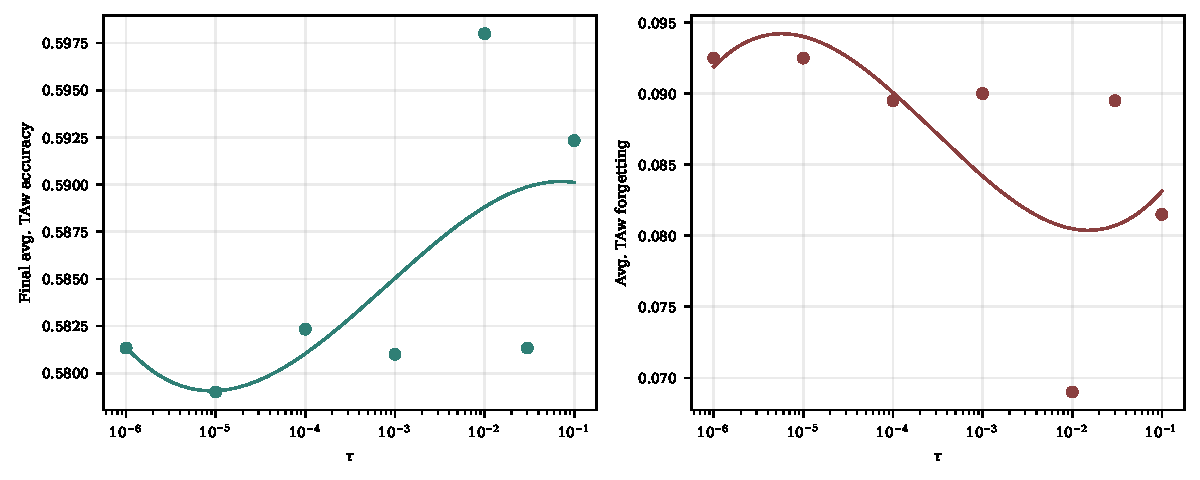
\includegraphics[width=0.62\linewidth]{figures/tau_sensitivity_cifar100.pdf}
\caption[Tau sensitivity on CIFAR-100]{Tau sensitivity on CIFAR-100. The tested values are $\{10^{-6},10^{-5},10^{-4},10^{-3},10^{-2},3\cdot10^{-2},10^{-1}\}$. The damping parameter has a measurable effect on this ResNet/FACIL prefix protocol: $\tau=10^{-2}$ gives the highest final task-aware accuracy and lowest forgetting among the tested values, so we use it as a practical default before task-specific tuning.}
\label{fig:tau-sensitivity-cifar100}
\end{figure}

\textbf{Effective Summand Norms} Figure \ref{fig:summand-norm-ecdf} reports a separate scale diagnostic from the original diagonal-analysis suite: CIFAR-100 classification, controlled regression, MNIST DDPM denoising, and the earlier binary segmentation setup. The plot shows the effective scale of the diagonal summands after multiplication by the corresponding $\lambda$. It is not a sample-weight plot, because the unweighted U-IEWC mechanism uses $h_n\equiv 1$.

\begin{figure}[H]
\centering
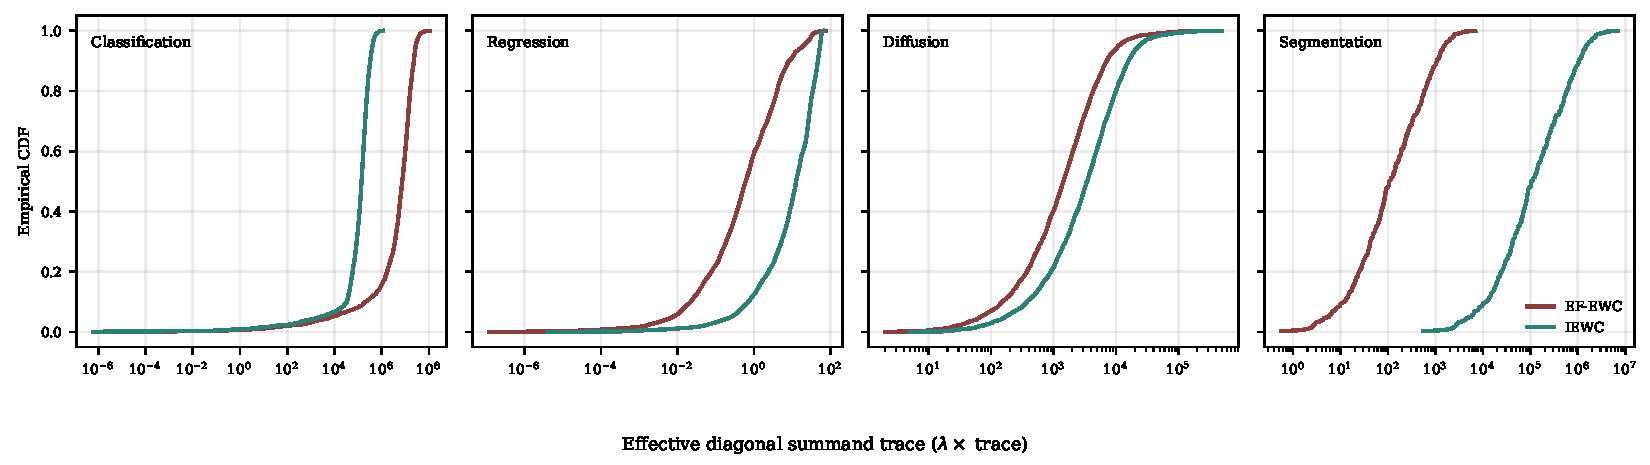
\includegraphics[width=0.95\linewidth]{figures/summand_norm_ecdf.pdf}
\caption[Effective diagonal summand norms]{Effective diagonal summand norms. Each panel reports the empirical CDF of $\lambda$ times the per-sample diagonal summand trace before averaging over old-distribution samples, with EF-EWC and IEWC shown on the same diagnostic task type.}
\label{fig:summand-norm-ecdf}
\end{figure}

For EWC-DR, we additionally checked $\lambda\in\{100,300,1000,3000,10000\}$ on the CIFAR-100 three-distribution prefix used for the damping plot. The best tested value on this prefix was $\lambda=100$; we use this only as a local parameter-sensitivity check for the earlier CIFAR-100 setup, not as the tuning protocol for the ImageNet-R results in Table \ref{tab:main-empirical-results}.
